\documentclass[main.tex]{subfiles}
\begin{document}

\chapter{Theory}
In this chapter theoretical concepts in quantum optics and quantum optimal control will be introduced.
First of, the quantum systems used in this thesis will be presented, then the cat code will be presented.
After that some important visualization tools for quantum mechanics are shown.
Finally, the basics of quantum optimal control are presented.
Note however that it is assumed that the reader has at least a basic understanding of quantum mechanics.

\section{Superconducting resonators}
Superconducting resonators are used in quantum computing both as the basis for qubits and as readout and control components \cite{}.
Although ideal resonators have equally spaced energy levels, in reality they are more or less anharmonic and the general Hamiltonian for a quantum anharmonic resonator is
\begin{equation}
    \Ham = \omega_{q} \au\ad + \frac{\kappa_q}{2} (\au)^2\ad^2
    \label{eq:resonator-hamiltonian}
\end{equation}
where \( \omega_{q} \) is the resonance frequency, \( \kappa_q \) is the anharmonic (self-Kerr) term and \(\ad\) is the destruction operator which removes an excitation from the resonator.
Note that this is still an approximation as higher order terms have been neglected.

The anharmonicity can be vizualised, see \cref{fig:anharmonic-energies}, by plotting the eigenenergies of \cref{eq:resonator-hamiltonian} as a function of \( \kappa \).
A larger anharmonicity makes the energy spacing larger for excitation states higher than \(\ket{1}\).
This anharmonicity is what permits a resonator to act as a qubit, as it is possible to adress only the first two states \( \ket{0} \) and \( \ket{1} \) due to the frequency difference.
Throughout this thesis, the term ``qubit'' will be used to refer to an anharmonic resonator even though it has more than two energy levels.
Further, the ``resonance frequency of the qubit'' which correspond to the energy spacing between the first two levels, will be referred to as \( \omega_{q} \).

\tikzfig{figs/energy-anharmonic}{The energy levels of a three-level resonator for anharmonicity \(\kappa\in[0,1]\) and \(\omega_{q}=1\).}{fig:anharmonic-energies}{25em}{20em}

\section{Coupled Qubit-Resonator System}
The Hamiltonian for a coupled qubit and resonator is chosen as
\begin{equation}
    \Ham(t) = \underbrace{\omega_{r}\au\ad + \frac{\kappa_r}{2}(\au)^2\ad^2}_{\text{Resonator}} + \underbrace{\omega_{q}\bu\bd + \frac{\kappa_q}{2}(\bu)^2\bd^2}_{\text{Qubit}} + \underbrace{g\qty(\au\bd+\ad\bu)}_{\text{Coupling}}
    \label{eq:hamiltonian-coupled}
\end{equation}
where \( \bd \) is the destruction operator for the qubit.
There is now a coupling term with the coupling strength \(g\) which means that the resonator and the qubit can exchange excitations between each other.
\(g\) will be assumed to be real for simplicity.
This is similar to the Jaynes-Cummings Hamiltonian, but now there are added self-Kerr terms for both the qubit and the resonator.
Another difference is that the Jaynes-Cummings model explicitly deals with a two-level qubit or atom, while this model has a ``qubit'' with arbitrary levels.
Note that the rotating wave approximation has been applied to the coupling term~\cite{wu_strong-coupling_2007}.

\section{Cat code}
\label{sec:cat-code}
The cat code is a logical basis for quantum information stored in resonators.
The basis states are
\begin{equation}
    \ket{0_L} = \cat{},\quad \ket{1_L} = \cat[i]{}
\end{equation}
where 
\begin{equation}
    \cat[(i)]{} = \frac{1}{\sqrt{2}}\qty(\ket{(i)\alpha} + \ket{-(i)\alpha}).
\end{equation}
That is the each basis state \( \ket{0(1)_L} \) in the cat code consists of a cat state \(\cat[(i)]{}\), which is a superposition of a coherent state \(\ket{(i)\alpha}\) and its negative counterpart \(\ket{-(i)\alpha}\).
A coherent state can be represented in the Fock basis as
\begin{equation}
    \ket{(i)\alpha} =\ex^{-{\frac{|(i)\alpha|^2}{2}}}\sum_{n=0}^{\infty}{\frac{\qty((i)\alpha)^n}{\sqrt{n!}}}\ket{n}.
\end{equation}
The basis can also be in an odd parity where the two coherent states are subtracted instead of added, however only the even parity basis will be used in this thesis.
A more detailed review of the cat code can be found in the supplementary information of~\cite{ofek_extending_2016}.
% TODO Explain what the cat code basis is and why it can be used for QEC.


\section{Visualization of quantum states}
In order to understand the results presented later in this thesis, some visualization techniques of quantum states are shown and explained.

\subsection{Bloch sphere}
\begin{figure}[H]
    \centering
    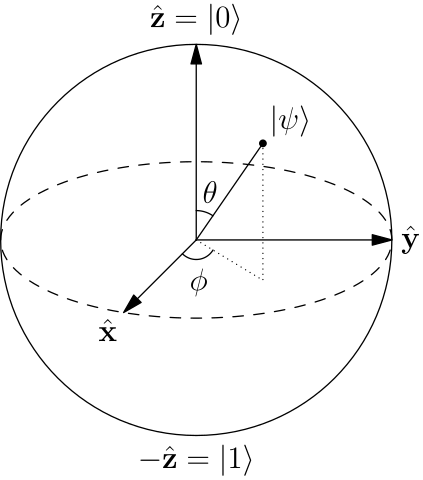
\includegraphics[width=0.3\textwidth]{figs/bloch_sphere.png}
    \caption{Representation of an abritrary pure quantum state on the Bloch sphere.
    \\ Source:~\cite{glosser.ca_english:_2012} (CC BY-SA 3.0).
    }%
    \label{fig:bloch_sphere}
\end{figure}

The pure state of a qubit can be visualized on the surface of a unit sphere with the following parametrization
\begin{equation}
    \ket{\psi} = \cos(\frac{\theta}{2})\ket{0} + \ex^{i\phi}\sin(\frac{\theta}{2})\ket{1}
\end{equation}
where \( \theta \) and \( \phi \) are angles which are shown in \cref{fig:bloch_sphere}.
The ground state \(\ket{0}\) is located on the ``north pole'' and the excited state \(\ket{1}\) on the ``south pole''.

Further, a handy trick to visualize the qubit when it has more levels than three is to ``project'' the state to the \(\qty{\ket{0},\ket{1}}\) basis with \( \op{0} + \op{1} \) and then plot it on the Bloch sphere.
This means that the subspace which is not spanned by the first two levels will be represented by the inside of the sphere.
To make an example, \(\ket{2}\) will lie right in the center of the sphere while \(\qty(\ket{1}+\ket{2})/\sqrt{2}\) will lie halfway between the center and the south pole.

%\subsection{Density matrices and Hinton diagrams}
%Even tough this thesis will only deal with pure quantum states \(\ket{\Psi}\) it can be interesting to look at the density matrix \(\op{\Psi}\).
%This density matrix can be visualized in a Hinton diagram which exposes the coefficients of the basis states of \(\ket{\Psi}\) in a visual way.
%This is a good way for quickly judging the quality of a quantum state.
% TODO Explain the Hinton diagram and density matrix

\subsection{Wigner function}
The wigner function can be used to visualize quantum states and processes.
It is a quasiprobability distribution where states exhibiting quantum phenomena will have negative values, impossible for classical states.

To give a visual example, 6 example states in the cat code basis are shown in \cref{fig:cat-resonator-wigner-targets} with \(\alpha=2\) and a Hilbert space size of \(N_r=8\).
Looking at \(\ket{0}\) we can see two lobes with an interference fringe in between them.
For large enough \(N_r\) there will be no truncation of the Hilbert space and the lobes will appear circular.
Compared to the basis states, the superposition states exhibit even more complex shapes.

\begin{figure}[ht]
	\centering
	\foreach \n/\capn [count=\ni] in {{0}/{\ket{0}},{5}/{\ket{1}},{3}/{(\ket{0}+\ket{1})/\sqrt{2}},{1}/{(\ket{0}-\ket{1})/\sqrt{2}},{2}/{(\ket{0}+i\ket{1})/\sqrt{2}},{4}/{(\ket{0}-i\ket{1})/\sqrt{2}}}{
		\subcaptionbox{\(\capn{}\)}{
			\centering
			\includegraphics[width=0.30\textwidth]{figs/cat_wigner_targets_\n.png}
		}%
		\ifnum\ni=6%
				%
		\else%
			\hfill
		\fi%
	}
	\caption{%
	Wigner function of some example states in the cat code basis with \(\alpha = 2\) and \(N_r=8\).
	}%
	\label{fig:cat-resonator-wigner-targets}
\end{figure}

% TODO Explain why the wigner function is good for visualization.

\section{Quantum optimal control}
Quantum control is the process of controlling a quantum system by controlling the amplitude of a set of control operators~\cite{fisher_optimal_2010}.
Such a system can be described~\cite{fisher_optimal_2010} by a Hamiltonian of the following form
\begin{equation}
    \Ham(t) = \underbrace{\Ham_d}_{\text{Drift}} + \underbrace{u_0(t)\Ham_0 + \dotsc + u_N(t)\Ham_N}_{\text{Control}}.
    \label{eq:optimal-control-hamiltonian}
\end{equation}
The controls are usually electromagnetic pulses changing in time and thus will be referred to as ``pulse shapes''~\cite{fisher_optimal_2010} in this thesis~.

There are two main questions in quantum control: one of \emph{controllability} and one of \emph{optimal control}.
The first deals with the \emph{existence} of solutions given a Hamiltonian and the second with the \emph{optimized} solutions for the pulse shapes \(\qty{u_i(t)}\)~\cite{dalessandro_introduction_2007}.
The optimal solutions are generally not analytically solvable and thus the pulse shapes need to be discretized in time and numerically optimized using algorithms.
The algorithm used for this thesis is called Krotov's method and will be presented in the Method chapter.

\subsection{Unitary transformation}
A unitary transformation can drastically simplify systems that are hard to simulate.
This idea will be conceptually presented here and then implemented in the Method chapter.
The transformation that is used is a special case of unitary transformations called the \emph{interaction picture} where the Hamiltonian is split up into a time-independent and time-dependent part
\begin{equation}
    \Ham(t) = \Ham_A + \Ham_B(t).
\end{equation}
By choosing the unitary operator \( \hat{U} = \ex^{i \Ham_A t} \) the unitary transformation takes us into the interaction picture
\begin{align*}
    \Ham &\rightarrow~ \hat{U}\qty[ \Ham_A  + \Ham_B(t)]\hat{U}^\dagger + i\dv{\hat{U}}{t}\hat{U}^\dagger =\\
    &=~ \hat{U}\Ham_A\hat{U}^\dagger + \hat{U}\Ham_B\hat{U}^\dagger + i\qty(i\Ham_A t)\ex^{i \Ham_A t}\ex^{-i\Ham_A t}=\\
    &=~ \Ham_A + \hat{U}\Ham_B\hat{U}^\dagger - \Ham_A = \hat{U}\Ham_B\hat{U}^\dagger
\end{align*}

\end{document}
